%!TEX root = skripsi.tex
%-----------------------------------------------------------------------------%
\chapter{\babTiga}
%-----------------------------------------------------------------------------%
Bab ini akan menjelaskan gambaran proses penelitian secara keseluruhan yang terdiri dari pembuatan \textit{sense tagged corpus} bahasa Inggris,  \textit{word alignment} korpus paralel, peningkatan kualitas dan evaluasi \textit{word alignment}, pemindahan \textit{sense} dari korpus bahasa Inggris, dan sistem WSD yang diimplementasikan. Diagram dari rancangan sistem yang akan dibuat pada penelitian ini dapat dilihat pada gambar berikut:

\begin{figure}
	\centering
	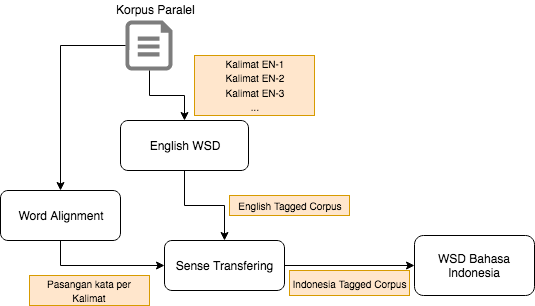
\includegraphics[width=1\linewidth]{adit_pics/WSD-full}
	\caption{Rancangan Sistem}
	\label{fig:Rancangan-Sistem}
\end{figure}
%-----------------------------------------------------------------------------%


\section{Korpus Identik}
Korpus utama yang digunakan sebagai sumber data penelitian ini adalah korpus identik. Korpus identik berisi pasangan kalimat-kalimat dalam bahasa Indonesia dan Inggris. Kalimat yang berpasangan di dalamnya sebagian besar mempunyai makna konten yang paralel walaupun terdapat juga yang \textit{comparable}. Korpus identik ini mempunyai 88.918 buah pasangan kalimat di dalamnya.


\section{Pembuatan \textit{Sense Tagged Corpus} Bahasa Inggris}
%-----------------------------------------------------------------------------%

Pembuatan \textit{sense tagged corpus} bahasa Inggris dilakukan dengan menggunakan \textit{tool} IMS untuk mendapatkan makna terbaik yang dapat ditag oleh \textit{tool} tersebut. Makna kata hasil dari proses ini akan dipindahkan ke kata yang bersesuaian pada kalimat yang sama pada bagian \textit{sense transfering}. \textit{File} yang diberikan sebagai masukan dari IMS adalah kalimat-kalimat pada bahasa Inggris yang berasal dari korpus identik.
%-----------------------------------------------------------------------------%
\section{\textit{Word alignment} pada Korpus Paralel}
%-----------------------------------------------------------------------------%
\textit{Word alignment} pada korpus berbahasa Inggris dan Indonesia menggunakan \textit{tools word alignment} bernama Giza++. \textit{Tool} ini merupakan salah satu \textit{word alignment tools} pada \textit{statistical machine translation} (SMT) yang dapat digunakan untuk memasangkan kata-kata pada dua buah korpus atau lebih. Terdapat beberapa \textit{word alignment tools} lain seperti Berkeley \textit{aligner}, anymalign, dan lain-lain. Penyelarasan kata ini digunakan untuk kebutuhan pemindahan \textit{sense} dari kata bahasa Inggris ke kata dalam bahasa Indonesia.

Proses \textit{alignment} yang dilakukan dengan Giza++ meliputi tahap-tahap berikut:
\begin{enumerate}
	\item Mempersiapkan kedua buah \textit{file} yaitu korpus bahasa asal (\textit{source}) dan korpus bahasa tujuan (\textit{target}). Kedua \textit{file} ini berpasangan dalam setiap barisnya. Baris pertama dalam \textit{file} pertama berpasangan dengan baris pertama pada \textit{file} kedua sampai akhir baris pada kedua \textit{file}.
	\item Menghasilkan \textit{file} perbendaharaan kata dari kedua bahasa dan \textit{list} indeks perbendaharaan kata pada tiap kalimat yang sudah diselaraskan
	\item Menghasilkan \textit{cooccurence file} dari kosa kata dan pasangan kalimat tersebut
	\item Proses \textit{alignment} yang menghasilkan beberapa macam \textit{output file} 
\end{enumerate}

Terdapat satu buah \textit{output file} Giza++ yang berisi pasangan-pasangan kalimat dengan kata-kata yang sudah diselaraskan dengan translasinya dalam bahasa tujuan. Hasil ini merupakan \textit{best viterbi alignment} menurut Giza++.

Pada skenario \textit{alignment} dengan bahasa Indonesia sebagai \textit{source} dan bahasa Inggris sebagai \textit{target}, satu kata dalam bahasa Indonesia akan dipasangkan dengan tepat satu kata dalam bahasa Inggris.

%-----------------------------------------------------------------------------%
\section{Evaluasi \textit{Word Alignment}} \label{sec:pembentukanTdanH}
%-----------------------------------------------------------------------------%
\textit{Word alignment} hasil dari \textit{tool} Giza++ dievaluasi dengan menggunakan \textit{anotator} hasil \textit{alignment} dari \textit{anotator} yang akan ditujukan sebagai \textit{gold standard}. Nilai-nilai yang akan dihitung meliputi \textit{precision} (P), \textit{recall} (R), dan F-\textit{score}. Metode evaluasi keseluruhan meliputi:

\begin{enumerate}
	\item Pemilihan \textit{random sampling} sebanyak dua ratus buah pasangan kalimat
	\item Masing-masing \textit{anotator} memasang-masangkan kata yang tepat pada masing-masing pasangan kalimat, dengan asumsi bahwa anotasi manusia sebagai \textit{gold standard}
	\item Hasil anotasi manusia dan keluaran dari \textit{tool} Giza dibandingkan untuk mendapatkan ketiga nilai P, R, F-Score, dan \textit{agreement} kedua anotator.
\end{enumerate}


%-------%
\section{Peningkatan Kualitas Hasil \textit{Alignment}}
%-----------------------------------------------------------------------------%
Proses peningkatan kualitas hasil alignment diperlukan untuk meminimalisir kesalahan pemasangan kata-kata pada proses sebelumnya. Permasalahan  yang terjadi adalah adanya pasangan-pasangan kata yang tidak benar seperti pada halnya kata "lapangan" misalnya yang  dipasangkan dengan kata dalam bahasa inggris \textit{field}, \textit{ground}, \textit{involved}, \textit{job}, \textit{program}, dan beberapa kata lainnya. Peningkatan kualitas \textit{alignment} ini dilakukan dengan dua buah pendekatan, yaitu dengan bantuan \textit{online dictionary} bahasa Indonesia-Inggris dan \textit{bi-directional alignment}. Pendekatan dengan bantuan kamus diterapkan dengan mencari kata terjemahan pada bahasa Inggris untuk menentukan apakah \textit{alignment} benar atau salah. Pada pendekatan kedua, dilakukan \textit{inverse} \textit{alignment} antara bahasa Indonesia ke Inggris. Jika pada proses awal \textit{alignment} dilakukan dengan menerapkan bahasa Indonesia sebagai \textit{source} dan Inggris sebagai \textit{target}, kali ini dilakukan proses yang berkebalikan. Pemanfaatkan hasil \textit{alignment} korpus bahasa Inggris ke Indonesia akan menghasilkan pasangan-pasangan kata dengan tingkat kesalahan \textit{alignment} lebih kecil dari \textit{alignment} satu arah saja. Metode yang akan dilakukan adalah dengan memeriksa setiap pasangan kata dari bahasa Indonesia yang mana merupakan kata dalam bahasa Inggris, apakah kata tersebut memiliki pasangan dalam \textit{inverse alignment} Giza.

%-----------------------------------------------------------------------------%
\section{\textit{Sense Transfering}} \label{sec:Sense Transfering}
%-----------------------------------------------------------------------------%
Pemindahan makna kata dilakukan dengan tiga buah \textit{sub-process} yang terdiri dari pemasangan antar kalimat, pemeriksaan kata, dan \textit{sense transfering}.
\begin{enumerate}
	\item Pemasangan antar kalimat yang bersesuaian dengan kata-kata yang berpasangan. Pada contoh kata "halaman" yang berpasangan dengan "courtyard", maka pasangan kalimat "Aku bermain di halaman" akan dipasangkan dengan kalimat "I play at the courtyard".
	\item Pemeriksaan untuk kata yang saling berpasangan dari hasil \textit{alignment} dan kamus hasil \textit{alignment enhancement}.
	\item \textit{Sense} dari kata yang menjadi \textit{target} tersebut kemudian diperiksa dengan \textit{sense} kata yang sama yang sudah pernah dipindahkan dari pasangan kalimat lain. 
	\item Jika \textit{sense} yang ingin dipindahkan "mirip" dan memiliki kedekatan makna dibatas \textit{threshold}, maka \textit{sense} yang akan dipindahkan hanya salah satu saja. Proses ini diperlukan untuk meminimalisir adanya satu kata bahasa Indonesia yang mempunyai lebih dari satu \textit{sense} yang mirip dari definisi makna tersebut.
	\item Bila "courtyard" memiliki \textit{sense} yang artinya adalah "halaman rumah", maka "halaman" pada kalimat "Aku bermain di halaman" memiliki \textit{sense} "halaman rumah".
\end{enumerate}

\section{Sistem WSD} \label{sec:Sistem WSD}
%-----------------------------------------------------------------------------%
Sistem WSD yang dibangun adalah dengan menggunakan pendekatan \textit{supervised learning}. Hasil dari pemindahan makna kata akan digunakan sebagai \textit{training} dan \textit{testing} data untuk menguji performa dari sistem yang dibangun. \textit{Classifier} yang digunakan dalam sistem \textit{WSD} ini adalah SVM. Pengujian dilakukan dengan menggunakan beberapa fitur seperti \textit{bag of words}, \textit{POS Tag}, dan \textit{word embedding}. Fitur \textit{bag of words} menggunakan \textit{window} sebanyak dua buah kata kanan dan kiri kata tujuan sebagai kata konteks. \textit{POS Tag} dan vektor \textit{word embedding} juga akan diimplementasikan pada penelitian ini. Performa dari sistem WSD akan dilihat berdasarkan perhitungan F1-score \textit{micro} dari hasil klasifikasi.